% File language.tex

% -*- Master-File: manual.tex; Document-Type: LaTeX -*- 

% [ck: Aug  9 95]
% \chapter{\elan: the language}

This chapter presents a full bottom-up description of the language
features that, contrary to Chapter~\ref{short}, uses a construction of
the language only when it has been introduced before.

The \elan\ syntax is given in the Extended Backus-Naur Form (EBNF). 
We assume that the reader is familiar with this well-known notation,
where for instance \itone{X} \mbox{(resp. \itzero{X})} denotes a non-empty
(resp. a possibly empty) repetition of X, and \omm{X} means that X is
optional, and may be omitted.

All examples given below are running under the current
implementation of the \elan{} version \versionElan{}.

\section{Lexicographical conventions}

\subsection{Separators}

All ASCII characters whose code are less or equal than 32 are
considered by the parser as \Def{separators}. Thus spaces, tabulations and
newlines are separators.

\subsection{Lexical unities}

A \Def{lexical unity} in \elan\ is either an identifier, a natural number
or a special character.

Identifiers are composed by concatenation of letters, numerals and the
character ``\sym\_'', and they  should begin with a letter.

\index{letter}
\grrule{letter}{\tt
A\sor B\sor C\sor D\sor E\sor F\sor G\sor H\sor 
I\sor J\sor K\sor L\sor M\sor N\sor O\sor P\sor Q\sor R\sor S\sor T\sor 
U\sor V\sor W\sor X\sor Y\sor Z 
\gror
 a\sor b\sor c\sor d\sor e\sor f\sor g\sor h\sor 
i\sor j\sor k\sor l\sor m\sor n\sor o\sor p\sor q\sor r\sor s\sor t\sor 
u\sor v\sor w\sor x\sor y\sor z
}

\grrule{numeral}{\tt
0\sor 1\sor 2\sor 3\sor 4\sor 5\sor 6\sor 7\sor 8\sor 9
}

\grrule{identifier}{ 
  \nt{letter} \itzero{\nt{letter} \sor \nt{numeral} \sor ~\sym{\_}}
}

\grrule{quoted identifier}{ 
  \sym{'}
  \itone{\nt{letter} \sor \nt{qchar} \sor \nt{numeral} \sor ~\sym{\_}} \sym{'}
}

\label{elan id}
\grrule{elan identifier}{
        \nt{identifier} {\sf except \elan's keywords}
}

All characters different from the previously introduced ones (letters,
numerals, separators) and the characters `\{', `\}', `$\tilde{\ }$',
are considered as special characters and are referenced as
\nt{char}.

\grrule{nchar}{
  \nt{char} {\sf except `@' and `:'}
}

\grrule{qchar}{
    \nt{char} {\sf except `\sym{'}'}
}

A \Def{number} is the concatenation of numerals.

\grrule{number}{ \itone{\nt{numeral}}}

\subsection{Comments}

All strings enclosed between the strings ``\verb|/*|'' and ``\verb|*/|'' or
between the string ``\verb|//|'' and the end of line, are considered by the
parser as \Def{comments}.


\section{Element modules}
\label{Element modules}

Element modules are the basic unit blocks of the language. They allow to
define computational systems i.e. to define a rewrite theory together
with a strategy. 
For modularity reasons, importations are made
possible in \elan\ modules, under the condition that no cycle exists
in the importation relation. This is described in the modularity
section~\ref{Modularity}. 

The syntax is the following:

\index{sort!definition}
\grrule{module}{
        \rw{module} \nt{formal module name} \nl
        \omm{\nt{imports}}              \nl
        \omm{\nt{sort definition}}      \nl
        \omm{\nt{operator definition}} \nl
        \omm{\nt{stratop definition}} \nl
        \itzero{\nt{family of rules}}   \nl
        \itzero{\nt{family of strategies}}      \nl
        \rw{end}
}


The module of name {\tt ModuleName} should be declared in the file {\tt
ModuleName.eln}. Only one, and exactly one module can be described in
a given file. 

Importations can be made local or global: 

\begin{tabbing}
$<${\em imports}$>$ \= {\tt ::=} \= {\bf import} {\tt \{ $<$}{\em
instantiated module name}$>$ {\tt \}$^{~+}$ \sym{;}} {\bf end} \\
\>{\tt |}\>{\bf import}  \omm{$<${\em global imports}$>$} \omm{$<${\em local imports}$>$} {\bf 
end}\\\\
%%%$<${\em global or local imports}$>$ \= {\tt ::=} \= {\bf global} {\tt 
%%%\{ $<$}{\em module name}$>$ {\tt \}$^{~+}$ \sym{;} [ $<$}{\em
%%%local imports}{\tt $>$ ]}\\ 
%%%\>{\tt |}\>{\bf local} {\tt \{ $<$}{\em module name}$>$ {\tt
%%%\}$^{~+}$ \sym{;}} \\ 
$<${\em global imports}$>$ \= {\tt ::=} \= {\bf global} {\tt \{ $<$}{\em 
instantiated module name}$>$ {\tt \}$^{~+}$ \sym{;}} \\\\
$<${\em local imports}$>$ \= {\tt ::=} \= {\bf local} {\tt \{ $<$}{\em 
instantiated module name}$>$ {\tt \}$^{~+}$ \sym{;}} \\
\end{tabbing}
An instantiated module name like \texttt{List[List[Int]]} is described 
by:

\grrule{instantiated module name}{
  \nt{identifier}
\gror
  \nt{identifier} 
        \sym{[} \= \nt{instantiated module name} \\
\>\>\> \itzero{\sym{,}\nt{instantiated module name}}
        \sym{]}
}

\noindent
Sorts are always global:

\index{name!sort}\index{sort!definition}\index{sort!name}
\grrule{sort definition} {
  \rw{sort}
  \itone{\nt{sort name}} \sym{;}
  \rw{end}
}

\noindent
but operators can be exported, and thus declared global, or just local
in which case they can be used only in the module where they are defined.


\index{operator definition}
\begin{tabbing}
{\tt $<$}{\em operator definition}{\tt $>$} \= {\tt ::=} \= {\bf op}\={\bf 
erators}\\
\>\>\> \omm{\nt{global operator definition}} \omm{\nt{local operator definition}}\\
\>\> {\bf end} \\
\\
{\tt $<$}{\em global operator definition}{\tt $>$} \= {\tt ::=} \= {\bf 
global} {\tt \{ $<$}{\em operator declaration}{\tt $>$} {\tt \}$^{~+}$ \sym{;}} \\ 
\\
{\tt $<$}{\em local operator definition}{\tt $>$} \= {\tt ::=} \= {\bf 
local} {\tt \{ $<$}{\em operator declaration}{\tt $>$} {\tt \}$^{~+}$ \sym{;}} \\ 

\end{tabbing}

And similarly for strategy operator definition:


\index{stratop definition}
\begin{tabbing}
{\tt $<$}{\em stratop definition}{\tt $>$} \= {\tt ::=} \= {\bf st}\={\bf ratop}\\
\>\>\> \omm{\nt{global stratop definition}} \omm{\nt{local stratop definition}}\\
\>\> {\bf end} \\
\\
{\tt $<$}{\em global stratop definition}{\tt $>$} \= {\tt ::=} \= {\bf 
global} {\tt \{ $<$}{\em strategy declaration}{\tt $>$} {\tt \}$^{~+}$ \sym{;}} \\\\
{\tt $<$}{\em local stratop definition}{\tt $>$} \= {\tt ::=} \= {\bf 
local} {\tt \{ $<$}{\em strategy declaration}{\tt $>$} {\tt \}$^{~+}$ \sym{;}} \\
\end{tabbing}
{\tt $<$}{\em family of rules}{\tt $>$}
is defined in Section~\ref{Definition of rules}.
{\tt $<$}{\em family of strategies}{\tt $>$}
is defined in Section~\ref{Definition of strategies}.

\section{Definition of signatures}

\elan\ is a multi-sorted language, and signatures are composed by the
definitions of the sorts and operators symbols. The operator syntax is
given in a mix-fix form which allows the super-user to define very
conveniently its own syntax.

\subsection{Sort declarations}

A \Def{sort declaration}\index{declaration!sort}\index{sort!declaration} is either
a sort name (an identifier) or a sort name followed by the list of
sort names it depends on:

\index{name!sort}\index{sort!name}
\grrule{sort name} {
  \nt{identifier}
 \gror
  \nt{identifier}\sym{[}\nt{sort name}\itzero{\sym{,}\nt{sort name}}\sym{]}
}

\EX
\sortname{bool, int, list[bool], 
pair[int,list[bool]], list[X]} are sort names in \elan.
\FEX

\REM
A sort name is always {\em global} in \elan. Two sort declarations using the
same sort name, will result in the creation of only {\em one} sort.
\FREM

\paragraph{Built-in sorts}\index{sort!built-in}

For efficiency, sorts could be defined as built-ins. See
section~\ref{les built-in} for details.

%\begin{enumerate}
%\item \sortname{bool} which refers to the standard booleans.  The
%        \elan\ module {\tt bool} that introduces this sort is
%        defined on page~\pageref{bool module}.\index{sort!bool}
%\item \sortname{ident} which refers to any identifier.  The
%        \elan\ module {\tt ident} that introduces this sort is
%        defined on page~\pageref{ident module}.\index{sort!ident}
%\item \sortname{int} which refers to the standard integers. The \elan\
%        module {\tt int} that introduces this sort is defined on
%        page~\pageref{integer module}.\index{sort!int}
%\item \sortname{double} which refers to the ``standard'' floating
%        point numbers provided by the C language. The \elan\ module
%        {\tt double} that introduces this sort is defined on
%        page~\pageref{double.module}.\index{sort!double}
%\end{enumerate}

\subsection{Operator declarations}

A \Def{function symbol}, also called \Def{operator}, is given either by
defining a new symbol together 
with its rank or by aliasing an existing operator. Optional properties can
be specified:

\index{declaration!function}\index{declaration!operator}
\grrule{operator declaration}{
  \nt{new operator declaration}
\gror
  \nt{operator alias}
}

\grrule{new operator declaration}{
   \nt{operator name} \sym{:} \nt{rank} \omm{ \itone{\nt{operator option}} }
}

\grrule{operator alias}{\nt{new operator declaration} \rw{alias} \nt{old operator name}\sym{:}}

In case of \Def{aliasing}, \nt{new operator declaration} is only another
name for the function symbol \nt{old name}. The {\it two\/} names are then
accessible and refer to the {\it same\/} object.

\Attention{The last alias defined is considered by the parser as
having the highest priority with respect to the previously defined
ones.}

\grrule{old operator name}{\nt{operator name}}

\grrule{operator name}{\nt{name}}

The name of a function symbol contains information that will be used
by the mixfix parser to read a term:

\grrule{name} {\itone{\nt{symbol}}}
\grrule{symbol}{
  \nt{single lexem}
\gror
  \sym{@}
\gror
  \nt{quoted single lexem}
\gror
  \sym{'$\backslash$}\nt{number}\sym{'}
}
\grrule{single lexem}{
  \nt{elan identifier}
\gror
  \nt{number}
\gror
  \nt{nchar}
}
\grrule{quoted single lexem}{
  \nt{quoted identifier}
}
where, as defined on page~\pageref{elan id}, \nt{elan identifier} is
any identifier except keywords. Notice that indeed keywords can be
used without their special meaning when placed between quotes.

The characters 
`\{', `\}', `$\tilde{\ }$'
are restricted to the pre-processor use. Thus they cannot be used in
any module, but they can be used in the specification file or in the
description of the query, since both are not pre-processed.
The  `:' character indicates the end of the name and the character `@'
is the place-holder for an operator `@'rgument. These two last
characters can be used with another semantics than their built-in one,
when placed between quotes.

A quoted number after the character `$\backslash$' represents the
definition of a character by its ascii code. This facility can be used
in order to add to the syntactic form of a term non-visible characters
or the characters `\{', `\}', `$\tilde{\ }$'.

Finally an operator declaration is achieved by defining
its \Def{rank}, which is just a list of sort names with optional
description of \Def{selectors}.

\grrule{rank}{
  \nt{sort name}
\gror
  \sym{(} \itone{\nt{sort name}} \sym{)} \nt{sort name}
\gror
  \sym{(} \itone{\nt{identifier} \sym{:} \nt{sort name}} \sym{)} \nt{sort name}
}

\EX With the two declarations:\\
{\tt \symdef{@ + @}     {( int int ) int}{}}
{\tt \aliasdef{+(@,@)}  {( int int ) int}{}     {@+@}}
the strings ``$\tt x+y$'' and ``$\tt +(x,y)$'' represent the same
term.
\FEX

When defining a constructor operator, it is possible to define the
related selectors and modifiers, as outlined in the next example.

\EX
In the following module example, the selector {\tt first} and {\tt second}
are specified and the system will automatically generate the
corresponding selector and modifier operators and the corresponding
rewrite rules.

\insertExamples{simplePairSelectors.eln}

\noindent
This is similar to the following module:

\insertExamples{simplePair.eln}

\noindent
where the following rewrite rules are in fact automatically generated:
\begin{verbatim}
 (x,y).first => x              
 (x,y).second => y
 (x,y)[.first<-z] => (z,y)     
 (x,y)[.second<-w] => (x,w)
\end{verbatim}

\FEX

\subsection{Function declaration options}

As in languages like OBJ or ASF+SDF, an operator declaration carries
many informations about the syntax and the semantics of the
operator. We also need to specify complementary information like the
precedence of the operator for the parser, or some of its semantic
properties like associativity. This is done in \elan\ using the
following syntax:

\index{assocLeft}\index{assocRight}\index{pri}\index{AC}\index{code}
\grrule{operator option}{
  \rw{assocLeft}
\gror
  \rw{assocRight}
\gror
  \rw{pri} \nt{number}
\gror
  \sym{(} \rw{AC} \sym{)}
\gror
  \rw{code} \nt{number}
\gror
  \rw{builtin} \nt{number}
}

\paragraph{Parsing Associative operators}
The first two options are useful for defining syntactic associativity
of symbols:

\EX
The declarations:\\
{\tt 
\symdef{@ * @}{( int int ) int}{\rw{assocLeft}}
\aliasdef{*(@,@)}{( int int ) int}{}{@*@}}
allow to parse the term $\tt x * y * z$ as $\tt *(*(x,y),z)$.
\FEX

\paragraph{Priorities}
The \Def{priority} parsing problems can be solved using the priority
option: 

\EX
The declarations:\\
{\tt 
\symdef{@ + @}{( int int ) int}{\rw{assocLeft} \rw{pri} 10}
\symdef{@ * @}{( int int ) int}{\rw{assocLeft} \rw{pri} 20}}
allow to parse an expression like $\tt x + y * z$ as usual in 
$\tt x + (y * z)$.
\FEX

\Def{Coercions} can be defined and even hidden as in the following
example:

\EX
Assume that equations are constructed with the equality symbol:\\
{\tt 
\symdef{@ = @}{( term term ) equation;}{}}
and equational systems as conjunctions of equational systems:\\
{\tt 
\symdef{@ \& @}{( eqSystem eqSystem ) eqSystem;}{}}
An equation should be considered as an equational system, 
which corresponds to consider the sort {\tt equation} as a subsort 
of {\tt eqSystem}. This is done by the declaration of an invisible
operator:\\ 
{\tt 
\symdef{@}{( equation ) eqSystem;}{}}
This (invisible) coercion allows parsing  the expression {\tt (P \& e)}
where {\tt P:eqSystem; e:equation}.

\FEX

\paragraph{Semantic properties}
Semantic properties can be used.  Currently only associativity and
commutativity (abbreviated \Def{AC}) is allowed and only for binary
operators. 
The user should be aware that in interpreted mode, AC matching 
can be quite inefficient. It  is strongly recommended to use the
compiled mode in presence of AC operators.
% Since in this case AC matching is performed during
% evaluation this can lead in efficiency problems, since AC-matching is
% NP-complete in case of non-linear patterns~\cite{BenanavKN-JSC87}.

\EX
One can define a union operator which is associative and commutative
in the following way:\\
{\tt \symdef{@ $\cup$ @}{( set set ) set}{(\rw{AC})}}
\FEX

\paragraph{User built-in operators}
In order to improve efficiency of the evaluation, built-in
operators can be specified using the \rw{code} and \rw{builtin}
options. The natural number specified after the \rw{code} and
\rw{builtin} keywords specifies the index of this symbol in the symbol
table of \elan. A \rw{builtin} option is for built-in operators
without attached code defining its semantics, while the \rw{code}
option is for built-in operators with an attached procedure.

\EX 
The symbol $\tt true$ is defined in the {\tt bool} module as the first
symbol of the symbol table:\\
{\tt \symdef{true}{bool}{\rw{builtin} 1}}
\FEX

Section~\ref{les built-in} summarizes the codes already
defined for \elan's standard built-ins.

\Attention{Adding built-in operators is of course a delicate matter
since the \elan\ source code has to modified.}


\subsection{Strategy declaration}

A \Def{strategy operator} is similar to a function symbol as defined
previously except that at least one of the sorts involved in the
strategy rank is a strategy sort. 

\index{declaration!strategy}
\grrule{strategy declaration}{
  \nt{new strategy declaration}
\gror
  \nt{strategy alias}
}

\grrule{new strategy declaration}{
   \nt{strategy name} \sym{:} \nt{strategy rank} \omm{\nt{strategy option}}
}

\index{alias!strategy}
\grrule{strategy alias}{\nt{new strategy declaration} \rw{alias} \nt{old strategy name}\sym{:}}

In case of \Def{aliasing}, \nt{new strategy declaration} is only another
name for the strategy operator \nt{old strategy name}. The {\it two\/} 
names are then accessible and refer to the {\it same\/} object.

\Attention{The last alias defined is considered by the parser as
having the highest priority with respect to the previously defined
ones.}

\grrule{old strategy name}{\nt{strategy name}}

\grrule{strategy name}{\nt{name}}

\index{rank!strategy}
% \grrule{strategy rank}{
%   \nt{strategy sort}
% \gror
%   \sym{(} \itone{\nt{strategy sort}} \sym{)} \nt{strategy sort}
% }  %%%% [ck: May  5 99]

\grrule{strategy rank}{
  \nt{strategy sort name} 
\gror
  \sym{(} \nt{strategy args}  \sym{)} \nt{sort name}
\gror
  \sym{(} \itone{\nt{strategy arg}} \sym{)} \nt{strategy sort name}
}

\grrule{strategy arg}{
 \nt{sort name}
\gror
 \nt{strategy sort name}
}

\grrule{strategy args}{
 \nt{sort name} \nt{strategy args}
\gror
 \nt{strategy sort name} \itzero{\nt{strategy arg}}
}

\index{sort!strategy}
\grrule{strategy sort name}{
  \sym{$<$}\nt{strategy sort name} \sym{\texttt{->}} \nt{strategy sort name} \sym{$>$}
\gror
  \sym{$<$}\nt{sort name} \sym{\texttt{->}} \nt{sort name} \sym{$>$}
\gror
  \sym{$<$}\nt{sort name} \sym{\texttt{->}} \nt{strategy sort name} \sym{$>$}
\gror
  \sym{$<$}\nt{strategy sort name} \sym{\texttt{->}} \nt{sort name} \sym{$>$}
}

\grrule{strategy option}{
  \nt{elementary strategy option}
\gror
  \nt{defined strategy option}
}

\grrule{elementary strategy option}{
\rw{bs}
}

\grrule{defined strategy option}{
  \rw{assocLeft}
\gror
  \rw{assocRight}
\gror
  \rw{pri} \nt{number}
\gror
  \sym{(} \rw{AC} \sym{)}
}

The \rw{bs} attribute (for {\bf b}asic {\bf s}trategy) indicates that
the definition of the strategy is given by a rewrite rule whose
right-hand side only uses the constructions of the elementary
strategies language defined in Section~\ref{ElementaryStrategies}.


\section{Definition of rules}
\label{Definition of rules}

Rewriting is the basic concept underlying the design of \elan. The
language allows defining labelled conditional rules with local
assignments. 
It is important to realize the difference between:
\begin{description}
\item[-- labelled rules] whose evaluation is fully controled by the user
  defined strategies and,
\item[-- unlabelled rules] which are intended to perform functional
evaluation.  
They are applied using a built-in left-most inner-most strategy.

\end{description}
A \Def{condition} controling the firing of a rule is a term of sort
{\tt bool} introduced by the {\bf if}\index{if} keyword.\\ A
\Def{local assignment} is introduced by the keyword {\bf where}. Its
main purpose is to assign to local variables the result of the
application of a strategy on a term.

\subsection{Rule syntax}
\label{Rule syntax}

Rules are introduced in families, possibly restricted to a single element.

\index{rules!labelled}\index{rules!unlabelled}\index{labelled
rules}\index{unlabelled rules}
\grrule{family of rules}{
        \rw{rules for} \nt{sort name}           \nl
        \omm{\itone{\nt{variable declare}}}     \nl
        \omm{\rw{global} \itone{\nt{labelled or unlabelled rule}}} \nl
        \omm{\rw{local}  \itone{\nt{labelled rule}}} \nl
        \rw{end}
}

\grrule{labelled or unlabelled rule}{
        \nt{labelled rule}
\gror   \nt{unlabelled rule}
}

\grrule{labelled rule}{
        \sym{[} \nt{rule label} \sym{]} \nt{rule body} \rw{end}
}

\grrule{rule label}{\nt{identifier}\omm{\sym{(} variable \itzero{\sym{,}\nt{variable}} 
                                        \sym{)}}}

\grrule{unlabelled rule}{
        \sym{[} \sym{]} \nt{rule body} \rw{end}
}


\grrule{rule body}{
        \nt{term} \sym{=$>$} \nt{term} 
        \sym{[} \itzero{\nt{if-where-choose}} \sym{]}
}

\grrule{if-where-choose}{
        \rw{if} \nt{boolean term}   
\gror   \rw{where} \nt{variable name} \sym{:=}
        \sym{(} \omm{\nt{Estrategy term}} \sym{)} \nt{term} 
\gror   \rw{where} \nt{variable name} \sym{:=}
        \sym{[} \nt{Dstrategy term} \sym{]} \nt{term} 
\gror   \rw{where} \sym{(} \nt{sort name} \sym{)} \nt{term} 
        \sym{:=} \sym{(} \omm{\nt{Estrategy term}} \sym{)} \nt{term} 
\gror   \rw{where} \sym{(} \nt{sort name} \sym{)} \nt{term} 
        \sym{:=} \sym{[} \nt{Dstrategy term} \sym{]} \nt{term} % \nlp{2}
\gror   \rw{choose}\nlp{5}
        \itone{\rw{try} \nt{if-where-choose} } \nlp{5}
        \rw{end}
}

\grrule{variable declare}{
        \omm{\itzero{\nt{variable name} \sym{,}} \nt{variable name}} \sym{:}
        \nt{sort name} \sym{;}}
\grrule{variable name}{\nt{elan identifier}}

\nt{Estrategy term} defined in Section~\ref{ElementaryStrategies}
is a constant strategy name declared with the attribute \rw{bs}.
Note that it is optional.

\nt{Dstrategy term} defined in Section~\ref{DefinedStrategies}
is a term built on the signature of strategy operators.

\REM
The syntax for terms is not defined here since it is user defined and
induced from the rank of the operators. Because of the very liberal
way of defining operator ranks, the term syntax in \textit{mixfix} in the
tradition of algebraic specification languages like ASF+SDF or
OBJ. The term parser is based on Earley's context free parser~\cite{Earley}
where the grammar is extracted from the operator rank definitions.
\FREM

\releaseNote{Since \texttt{V.3.0}, the choose-try construction,
the patterns in where facility and the user defined strategies call by
``\texttt{[ ]}'' have been introduced.

The rule labels accept now arguments that should be variables used in
the rule.

%This version inherits of two syntactic features that are not
%completely satisfactory but that cannot be changed
%straightforwardly. The first one is the way to introduce a sort for a
%pattern in the {\bf where} part: in the form {\bf where}
%({\it sort}) {\it term}..., {\it sort} is just used to declare the
%sort of the term before parsing it. The current syntax should not be
%confused with a strategy call. 

In the {\bf where} construction with a term, the sort is just used to
declare the sort of the term used as pattern. This is useful for the
parser which then just checks that this is also the sort of the result
on the right hand side of ``\rw{:=}''. Note that the sort declarations
is useless for the {\bf where}
construction using only variables, since the sort of the variable is always
attached to it.

%The second one comes from the fact that
%strategies can be applied using the operator \mbox{``( )''} 
%or \mbox{``[ ]''}. This
%is mainly due to historical reasons and to the fact that we want to
%preserve downward compability and the efficiency of strategy evaluation.
}

There are two ways for calling strategies, according to the
strategy language used by the programmer:

\Attention{A strategy call of the form ``( )'' can only be done using a
strategy that is declared as \rw{bs}.}

\Attention{A strategy call of the form ``[ ]'' can only be done using a
strategy that is {\it not\/} declared as \rw{bs}.}

\EX
Here is one way for defining the idempotency rules for
booleans. Notice that the two rules are local to the module so
that their label can only be used for defining strategies in this
module. Note also that the two rules have, on purpose, the same
label:
\insertExamples{rule-ex.eln}
\FEX

Since several rules may have the same label, the resulting ambiguities
are handled by the strategy evaluation as explained later. The rule
label is optional and rules may have no name. This last case is
designed in such a way that the intended semantics is functional, and
it is currently the responsability of the rewrite rule designer to
check that the rewrite system composed of all unlabelled rules is
confluent and terminating.  Unlabelled rules are handled by a built-in
strategy (left-most inner-most) as fully described in
Section~\ref{Evaluation mechanism}.

\subsection{The where construction}\index{where}
\label{subsec.where.construction}

The {\bf where} construction has several purposes. The first one is to
modularize the computations by computing auxiliary results affecting
them to local variables, thus providing computation sharing. The
second is to direct the evaluation mechanism using strategies and the
built-in left-most inner-most evaluation reduction. Let us review the
possibilities offered by \elan.

The {\bf where} statement is first useful when one wants to
call a strategy on subterms.

\EX As a first introducing example, let us consider the module:
\insertExamples{ruleWithWhere.eln}

Using the rule {\tt r0}, the term {\tt a} reduces in one step to {\tt
b}. Using the rule {\tt r1}, the term {\tt b} is first normalized into
{\tt b'} using unlabelled rules and then {\tt a} is replaced by {\tt
b'}.  Using the rule {\tt r2}, the term {\tt b} is first normalized
into {\tt b'} using unlabelled rules and then the strategy {\tt
strat}, defined elsewhere by the super-user, is applied on {\tt b'}
and the result is substituted to {\tt a}.

\FEX

One can also perform more complex affectations of the local variables
by using \Def{patterns}.

The current syntax of the {\bf where} statement with patterns
\index{where!with pattern} \index{pattern!in where}\index{sort!in pattern} can be
rephrased as follows:
\[
  {\bf ~where~} (sort)p ~::= ()term ~|~ (s)term ~|~ [s]term
\]
where the pattern $p$ should be of sort $sort$.
AC-operators as well as non-linearity are allowed for patterns.

This pattern in where capability is exemplified in the next
subsection.

\subsection{Choose-Try}\index{choose-try}

The construction {\bf Choose try} allows factorizing common parts of 
rules with the same left-hand side.
For instance the two rules
$$ 
\begin{array}{llllllll}
& [\ell] & l & \Rightarrow & r & 
        {\bf where}\ y_1 := ()u_1  \\
&&&&&   {\bf if}\ c'_2(l,y_1) \\
&&&&&   {\bf where}\ y_3 := ()u_3  \\
& [\ell] & l & \Rightarrow & r & 
        {\bf where}\ y_1 := ()u_1 & \\
&&&&&   {\bf if}\ c''_2(l,y_1) \\
&&&&&   {\bf where}\ y_3 := ()u_3  
\end{array}
$$
are factorized into one rule:
$$ 
\begin{array}{llllllll}
& [\ell] & l & \Rightarrow & r & 
        {\bf where}\ y_1 := ()u_1 & \\
& & & & & {\bf choose} \\
& & & & & \quad
        {\bf try}\ {\bf if}\ c'_2(l,y_1) \\ 
& & & & & \quad
        {\bf try}\ {\bf if}\ c''_2(l,y_1) \\
& & & & & {\bf end} \\
&&&&&   {\bf where}\ y_3 := ()u_3  
\end{array}
$$
%
In this factorized form, the term $u_1$ is normalized only once
and the assignment to $y_1$ is performed also only once.

\EX

This example shows the use of patterns as well as the {\bf Choose try}
construction.

%%%%CHANGER L'EXEMPLE 
%%%\fbox{[pem: Nov 26 98] Je pense que cela ne tourne pas}

\insertExamples{quick.eln}

\FEX

%\subsection{Switches}\index{switch}
%
%When specifying with conditional rewrite rules, one of the syntactic
%difficulty is to write a family of rewrite rules in such a way that
%the disjunction of the conditions covers all the possible cases. The
%{\bf switch} construction in \elan\ intends to facilitate such a
%writing:
%
%\[\begin{array}{ll}
% l \Rightarrow  & \quad whifs \\
%                & {\bf switch~} \\
%            & \quad {\bf ~case~} c_1 {\bf ~then~} r_1 \quad whifs_1 \\
%            & \quad \dots \quad \dots \quad \dots \quad \dots\\
%            & \quad {\bf ~case~} c_n {\bf ~then~} r_n \quad whifs_n \\
%            & \quad {\bf ~otherwise~}  \quad ~r_0 \quad whifs_0 \\
%            & {\bf ~end~} \\
% {\bf ~end~}
%\end{array}\]
%where the sequence of wheres and ifs is defined as follows:
%\[
% whifs     ::= \{ {\bf ~where~} affectation  ~|~ {\bf ~if~} c \}^{*}
%\]
%
%\noindent
%As expected, the semantics of the {\bf switch} construction is the following:
%\[\begin{array}{lll}
%  l \Rightarrow & r_1 \quad (whifs \quad ({\bf ~if~} c_1 & whifs_1)) \\
%  l \Rightarrow & r_2 \quad (whifs \quad ({\bf ~if~} c_2 {\bf ~if~} not(c_1) & whifs_2)) \\
%            & \quad \quad \dots \\
%  l \Rightarrow & r_n \quad (whifs \quad ({\bf ~if~} c_n {\bf ~if~} not(c_{n-1}) {\bf ~if~} not(c_1) 
%                         & whifs_n))\\
%  l \Rightarrow & r_0 \quad whifs &  whifs_0\\
%\end{array}\]
%which means that:\\
%--- either $c_1$ is true in which case $l$ rewrites to $r_1$,\\
%--- or $c_1$ is false and $c_2$ is true in which case $l$ rewrites to $r_2$,\\
%--- or $c_1$ and $c_2$ are false and $c_3$ is true in which case $l$ rewrites to $r_3$,\\
%--- $\cdots$ \\
%--- else $l$ rewrites to $r_0$.
%
%\noindent
%The construction {\bf ~switch~} is recursive.
%


\subsection{Conditions}

The boolean term $c$ given in a condition is reduced using the
strategy that results from normalization using the non labelled rules
and by the user defined strategies. If the computation stops and the
resulting term is the boolean {\bf true} then the condition is
considered to be satisfied and the rule can be applied. If the
computation stops and the resulting term is not {\bf true} then the
condition is considered as false.

\subsection{Labels visibility}
\index{visibility!rule labels}

The {\bf global} and {\bf local} attributes make sense only for
labelled rules. When a labelled rule is:
\begin{description}
\item[-- local,] then its label can only be used in the module in which
  the rule is declared,
\item[-- global,] then its label can be used in all the modules importing
  the module defining the rule, with the visibility described in the
  section on modularity (see section~\ref{Modularity}).
\end{description}

\Attention{According to their semantics, unlabelled rules are always global.}

\releaseNote{Since version V.3.0, the notion of single rule has
  been removed and the notion of rule locality has been introduced, so
  that rule labels can now be declared to be local to a module or, on
  the contrary, globally accessible. See section~\ref{versionChanges}
  for details concerning these changes.}

\REM 
We will see next on page \pageref{for each} how rule families can
be constructed automatically in \elan\ using the pre-processor
construction ``{\sc for each}''.

\FREM

\section{Definition of strategies}\label{Definition of strategies}

The notion of strategy is one of the main originalities of \elan.
In practice, a strategy is a way to describe which rewrite
computations the user is explicitly interested in. It specifies when a
given rule should be applied in the term to be reduced.  From a
theoretical point of view, a strategy can be viewed either as a
function or as a subset of all proof terms defined by the current
rewrite theory. The application of a strategy to a term results in the
(possibly empty) collection of all terms that can be derived from the
starting term using this strategy~\cite{KirchnerKV-MIT95,VittekThese}.
When a strategy returns an empty set of terms, we say that it {\em
fails}\index{fail!strategy}\index{strategy!failure}.

\Attention{A strategy enumerates all the terms it describes, should
  this collection be finite or not. Consequently the user should note
  that in case (s)he writes a strategy that enumerates an infinity of
  terms, then the evaluation process will of course not terminate.}

%\Attention{We distinguish (at least historically) between {\em elementary
%strategies} and {\em defined strategies}. The first ones are described in
%the next section and are mainly based on regular expressions, while the
%latter allow the user to define his own elaborated strategies.}

Two strategy languages are offered in \elan.  The language of \Def{elementary
strategies} \index{strategy!elementary} is mainly based on regular expressions
built from rule labels, while the language of \Def{defined strategies}
\index{strategy!defined} allows the user to define his own elaborated
strategies, possibly recursively.  Although the language of defined strategies
embeds all the constructions of the language of elementary strategies, the
latter is maintained since it is based on a more efficient implementation.

Families of strategy rules are intended to give a semantics to
the strategy operators.
The syntax of strategy rule families is the following:

\index{strategy}\index{strategy!family}
\grrule{family of strategies}{
        \rw{strategies for} \nt{sort name} \nl
        \omm{\itone{\nt{strategy variable declare}}}           \\
\> \itone{ \>
             \rw{implicit} \itone{\nt{elementary strategy rule}}
\gror        \rw{implicit} \itone{\nt{defined strategy rule}}
\gror        \rw{explicit} \itone{\nt{defined strategy rule}} } \nl
        \rw{end}
}

\grrule{strategy variable declare}{
        \omm{\itzero{\nt{variable name} \sym{,}} \nt{variable name}} \nl
         \sym{:} \nl
          \nt{sort or strategy sort name} \sym{;}
}

\grrule{sort or strategy sort name}{
        \nt{sort name} 
\gror   \nt{strategy sort name}
}

The keyword \rw{explicit} is only used with defined strategies and 
introduces a strategy rule that contains explicitly in its left-hand
side the application operator  $[@]@$ that will be introduced 
in Section~\ref{DefinedStrategies}.
Otherwise, the strategy rule is introduced by the keyword
\rw{implicit}.

\subsection{Elementary strategies syntax}
\label{ElementaryStrategies}.

The general syntax of elementary strategy rules is the following:

\index{elementary strategy}\index{strategy!elementary}
\grrule{elementary strategy rule}{
        \sym{[]} \nt{Estrategy name} \sym{=$>$} \nt{Estrategy term} \rw{end}\nl
}

An elementary strategy rule has no label. Thus it is always global.

\grrule{Estrategy term}{
       \nt{Estrategy name}
\gror  \nt{choosing}
\gror  \nt{concatenation}
\gror  \nt{iterator}
\gror  \nt{normalize}
\gror  \nt{normalize with trace}
\gror  \rw{fail}
\gror  \rw{id}
}

\grrule{choosing}{
       \rw{dc} \sym{(} \nt{Estrategy term} 
                \itzero{\sym{$,$} \nt{Estrategy term}} \sym{)}
\gror  \rw{dk} \sym{(} \nt{Estrategy term} 
                \itzero{\sym{$,$} \nt{Estrategy term}} \sym{)}
\gror  \rw{first} \sym{(} \nt{Estrategy term} 
                \itzero{\sym{$,$} \nt{Estrategy term}} \sym{)}
\gror  \rw{dc one} \sym{(} \nt{Estrategy term} 
                \itzero{\sym{$,$} \nt{Estrategy term}} \sym{)}
\gror  \rw{first one} \sym{(} \nt{Estrategy term} 
                \itzero{\sym{$,$} \nt{Estrategy term}} \sym{)}
}

\grrule{concatenation}
  {\nt{Estrategy term} \sym{;} \nt{Estrategy term}}

\grrule{iterator}{
       \rw{iterate*} \sym{(} \nt{Estrategy term} \sym{)} 
\gror  \rw{iterate+} \sym{(} \nt{Estrategy term} \sym{)} 
\gror  \rw{repeat*} \sym{(} \nt{Estrategy term} \sym{)} 
\gror  \rw{repeat+} \sym{(} \nt{Estrategy term} \sym{)} 
}

\grrule{normalize}{
       \rw{normalize} \sym{(} \nt{Estrategy term} \sym{)}
\gror  \rw{normalise} \sym{(} \nt{Estrategy term} \sym{)}
}

\grrule{normalize with trace}{
\rw{normin} \sym{(} \nt{Estrategy name} \itzero{\sym{$,$} \nt{Estrategy name}} \sym{)}
}

\noindent
\nt{Estrategy name} is a constant strategy name declared 
with the attribute \rw{bs}.

%\releaseNote{With respect to version 1.17, the $\|$ separator is
%replaced with a simple comma ``{\bf ,}''.}

\subsubsection{Labelled rules}

A labelled rule is the most elementary strategy and is called a \Def{primal
strategy}. \index{strategy!primal}

The application of a rewrite rule in \elan\ yields a set of results. There are
in general several ways to apply a given conditional rule with local
assignments.  This is first due to equational matching (e.g.  AC-matching) and
second to the {\bf where} assignment, since it may itself recursively return
several possible assignments for variables when using for example
non-deterministic strategies.

Note that there may be several rules with the same label.  If no rule
labelled~$\ell$ applies on the term $t$, the set of results is empty and we say
that the rule $\ell$ fails.

A labelled rule $\ell$ can be considered as the simplest form of a strategy
which returns all results of the rule application.

Thus the language provides basic constructions to handle this non-determinism
through choice strategy operators.


\subsubsection{Choice strategy operators}

Let us first concentrate on expressing choices among the set of
results on a primal strategy $\ell$.  By default the strategy $\ell$
returns all results of this primal strategy.  If at most one result is
needed, $\ell$ has to be encapsulated by the strategy operator 
{\bf dc one} that returns a non-deterministically chosen result, or 
{\bf first one} that returns the first result, when it exists.

\EX Let us consider the following module (incompletely described here):
\insertExamples{indeterminism.eln}

The application of the rule {\tt extractrule} on the term {\tt
empty U a U b} can be done in two ways, since the AC-matching
algorithm returns a complete set of matches consisting in the two
substitutions: 
{\tt \{ S $\mapsto$ empty U a, e $\mapsto$ b\}} and
{\tt \{S $\mapsto$ empty U b, e $\mapsto$ a\}}.

Using the strategy {\tt extractrule} on this term results in the set
consisting of two terms {\tt a} and {\tt b}.
\rw{dc one}({\tt extractrule}) returns either {\tt a} or {\tt b} depending 
of the implementation of the non deterministic choice.
\rw{first one}({\tt extractrule}) returns either {\tt a} or {\tt b} depending 
of the implementation of the AC-matcher.

\FEX

More choice operators are defined and apply in general on a list of arguments.

\begin{itemize}
\item The \dk\ operator, with a variable arity, is an abbreviation 
of \textit{dont~know~choose}. $\dk(S_1,\ldots,S_n)$ takes all strategies 
given as  arguments, and returns, for each of them the set of all its results.
$\dk(S_1,\ldots,S_n)$ fails if all strategies $S_1,\ldots,S_n$ fail.

\item The \dc\ operator, with a variable arity, is an abbreviation 
of \textit{dont~care~choose}. $\dc(S_1,\ldots,S_n)$ selects only one strategy
that does not fail among its arguments, say $S_i$, and returns all its results.
$\dc(S_1,\ldots,S_n)$ fails if all strategies $S_1,\ldots,S_n$ fail.
How to choose $S_i$ is not specified.

\item A specific way to choose an $S_i$ is provided by the \first\
operator that selects the first strategy
that does not fail among its arguments, and returns all its results.
So if $S_i$ is selected,  this means that all strategies
$S_1,\ldots,S_{i-1}$ have failed.
Again $\first(S_1,\ldots,S_n)$ fails if all strategies $S_1,\ldots,S_n$ fail.

\item If only one result is wanted, one can use the operators
\firstone\ or  \dcone\  that select a non-failing strategy among 
their arguments (either the first or anyone respectively), and return
a non-deterministically chosen result of the selected strategy.
\end{itemize}

%%%According to the previous definitions, when the list of strategy is
%%%reduced to one labelled rule, one can notice that
%%%the strategies $\ell$, $\dc(\ell)$, $\first(\ell)$ and $\dk(\ell)$
%%%are all equivalent in the sense that they return the same set of results.

\EX \label{testStrat.eln}
Consider the following module:\\
\insertExamples{testStrat.eln}

Then the strategy {\tt strat} applied to {\tt a} results in {\tt c},
and the same strategy applied to {\tt b} results in {\tt \{e,f\}}.

\FEX

Note that the same rule label can be used for naming
different rules. In fact this is equivalent to design rules
with different labels and a choice operator to link them.
For instance in Example~\ref{testStrat.eln}, we could have
the label {\tt r3} again instead of {\tt r4} for the fourth rule.
The strategy could then be defined as
{\tt dc(dk(r1), dk(r2), dk(r3))}.



\subsubsection{Strategies concatenation}

Two strategies are concatenated by applying the second strategy on
all the results of the first one.

The concatenation operator denoted ``\texttt{;}'' builds the sequential 
composition of two strategies $S_1$ and $S_2$. The strategy 
$S_1 ; S_2$ fails if $S_1$ fails, otherwise it returns all results
(maybe none) of~$S_2$ applied to the results of~$S_1$;


\EX In the same context as in the previous example
(Example~\ref{testStrat.eln}), the strategy:
\insertExamples{testConc.eln}

\noindent 
when applied on the term {\tt a} results in the application of first
{\tt r1}, then {\tt r5}, and finally  {\tt r3} and {\tt r4}
in all possible ways, yielding the results {\tt \{e,f\}}.
\FEX

\subsubsection{Strategy iterators}

In order to allow for the automatic concatenation of the same strategy,
\elan\ offers four powerful iterators:
%\indexMC{iterate}\indexMC{repeat*}\indexMC{repeat+}
%\grrule{iterator}{
%       \rw{iterate} \sym{(} \nt{strategy} \sym{)} 
%\gror  \rw{repeat*} \sym{(} \nt{strategy} \sym{)} 
%\gror  \rw{repeat+} \sym{(} \nt{strategy} \sym{)} 
%}

The strategy \rw{iterate*} corresponds to applying zero, then one, then
two, ... $n$  times the strategy to the starting term, until the strategy
fails. Thus (\rw{iterate*}({\tt s})){\tt t} returns $\tt \bigcup_{n =
0}^{\infty} (s^{n})t$. Notice that \rw{iterate*} returns the results
one by one, even when the iteration of the strategy never fails.
This strategy cannot fail since it returns at least the initial term.

Its variant \rw{iterate+} does not return the initial term but returns
$\tt \bigcup_{n = 1}^{\infty} (s^{n})t$. It can fail if $s$ fails 
on the initial term.

The strategy \rw{repeat} iterates the strategy until it fails and
returns just the terms resulting from the last unfailing call of the
strategy. The two variants are thus defined as:\\
(\rw{repeat*}({\tt s})){\tt t} = $\tt (s^n)t$ where $\tt (s^{n+1})t$
fails, $\tt n \geq 0$ and ${\tt s^0} = id$,\\
(\rw{repeat+}({\tt s})){\tt t} = $\tt (s^n)t$ where $\tt (s^{n+1})t$
fails and $\tt n > 0$.

\EX

%%%%%%A CHANGER 

To illustrate the basic behaviour of the elementary strategies, let us
consider the following module:
\insertExamples{stratFail.eln}

When applying the strategies on the terms \texttt{a} or \texttt{b}, we
are obtaining the following results:\\ 
\begin{center}
{\tt \begin{tabular}{|l||l|l|}
\hline
{\rm strategy}& a     & b             \\
\hline
tryIt   & \{b\} & $\emptyset$   \\
\hline
repeatS & \{b\} & \{b\}         \\
\hline
repeatP & \{b\} & $\emptyset$   \\
\hline
\end{tabular}}
\end{center}
In particular, the difference between the {\bf repeat*} and {\bf
repeat+} is due to to fact that when {\tt dc(a2b)} is applied
zero time, this is by definition the identity strategy, returning the
initial term.

\FEX

\EX The extraction of the elements of a list can be realized in the
following way: 
\insertExamples{iterRepeat.eln}

We then obtain the following results for the different strategies applied on the terms
\texttt{1} or \texttt{element(1.2.3)} respectively:\\
\begin{center}
{\tt \begin{tabular}{|l||l|l|}
\hline
{\rm strategy}        & 1             & element(1.2.3)        \\
\hline
all0    & $\emptyset$   & \{1, element(2.3)\}   \\
\hline
allRepS & 1             & \{1, 2, 3\}   \\
\hline
allRepP & $\emptyset$   & \{1, 2, 3\}   \\
\hline
allIter & 1             &  \{element(1.2.3), element(2.3), element(3), 1, 2, 3\}\\
\hline
\end{tabular}}
\end{center}

\FEX

\subsubsection{The normalize strategy}

Since labelled rules are applied only at the top of the
terms, it is useful to have at hand a way to apply a family of
labelled rules everywhere in a term to get it normalized. This is
provided in \elan\ by the {\bf normalize} strategy. This strategy
takes a strategy and use it in order to normalize the term on which it
is applied.

\Attention{There is no assumption of the way the rules are applied,
e.g. neither innermost nor outermost.}

\EX

A typical example of the use of {\bf normalize} is the normalization
process of the typed lambda calculus, whose main module is described
as follows:\\
\insertExamples{normLambda.eln}

\FEX

\subsubsection{The normalize strategy with trace}
This new strategy (\rw{normin}) normalizes terms with respect to a set of labelled rules in leftmost-innermost fashion.
Moreover, a complete trace is generated (see option \verb|-proofterm| of the compiler).
This trace contains all informations about each rewrite step ({\it i.e.}
the context, the rule and the substitution) and allows the
normalisation process to be exported to external systems. The
strategy \rw{normin} is used, for example in an {\elan} based tactic for
(simple or AC) rewriting in the {\coq} proof assistant available
at~\cite{ACCoqELAN}.

\subsubsection{Identity and Failure}

Two more  constructions are available:

\begin{itemize}
\item $\id$ is the identity strategy that does nothing, and never fails.

\item $\fail$ always fails and returns an empty set of results.
\end{itemize}


\subsection{Defined strategies}
\label{DefinedStrategies}

The defined strategy language extends the elementary one by the possibility to
define recursive strategies.
The application of a defined strategy is itself performed by an \elan\ program
that defines the interpretation of the new constructions introduced by
the user.  All the modules defining the appropriate syntax and
semantics are provided in the \elan\ library.

%%%\fbox{Revoir les 2 paragraphes suivants [ck: Nov 23 98]}

The syntax of the defined strategy language is described in an \elan\ module
called {\tt strsig[X,Y]} when strategies ranks contain sorts of the form {\tt
<X->Y>} (strategies are non sort-preserving), and the module {\tt
strat[X]} when the strategies concern sorts of the form {\tt <X->X>}
(strategies are sort-preserving). To use non sort-preserving
strategies, one has to import the module {\tt tcstrat[X,Y]} where {\tt
X} and {\tt Y} are different sorts. These modules implement the
interpreter of the defined strategy language using a set of labelled
rewrite rules and a basic strategy {\tt eval}. The syntax of defined
strategies is given below: 

\index{strategy!defined}\index{defined!strategy}
\grrule{defined strategy rule}{
        \gror \sym{[\rule{1.65mm}{0mm}]} \nt{strategy body} \rw{end}\nl
        \gror \sym{[.]} \nt{strategy body} \rw{end}\nl
        \gror \sym{[} \nt{rule label} \sym{]} 
                \nt{strategy body} \rw{end}\nl
}

\grrule{strategy body}{
        \nt{Dstrategy term} \sym{=$>$} \nt{Dstrategy term} 
        \omm{\itone{\nt{if-where-choose}}}
}

%\grrule{if-where-choose}{
%        \rw{if} \nt{boolean term}   
%\gror   \rw{where} \nt{var name} \sym{:=}
%        \sym{(} \omm{\nt{Estrategy term}} \sym{)} \nt{term} 
%\gror   \rw{where} \nt{var name} \sym{:=}
%        \sym{[} \nt{Dstrategy term} \sym{]} \nt{term} 
%\gror   \rw{where of sort} \sym{(} \nt{sort name} \sym{)} \nt{term} 
%        \sym{:=} \sym{(} \omm{\nt{Estrategy term}} \sym{)} \nt{term} 
%\gror   \rw{where of sort} \sym{(} \nt{sort name} \sym{)} \nt{term} 
%        \sym{:=} \sym{[} \nt{Dstrategy term} \sym{]} \nt{term} \nlp{2}
%\gror   \rw{choose}\nlp{5}
%        \itone{\rw{try} \nt{if-where-choose} } \nlp{5}
%        \rw{end}
%}

\noindent \nt{if-where-choose} is defined in Section~\ref{Rule syntax}.

\noindent \nt{Dstrategy term} is a term built on the signature of strategy
operators. It has a strategy sort.

\noindent The different labels $\sym{[]}$, $\sym{[.]}$ and $\sym{[\ell]}$
for strategy rules correspond to different evaluation modes
explained in Section~\ref{Rewrite rules on strategies}.

\EX

An example of the use of these features is the following:
\insertExamples{map.eln}

\FEX

\EX
The following module shows how to program loops with the defined
strategy language.

\insertExamples{loop.eln}


\FEX


\section{Evaluation mechanism}\label{Evaluation mechanism}
\index{evaluation!mechanism in \elan}

This section does not introduce any new syntactic material, but gives
informal explanations on the operational semantics of the
language.
% For a full description of the operational model, the reader
%is invited to consult~\cite{ElanOPSem97}.

\subsection{Rewrite rules on terms}

As we have seen, there are two kinds of rules: labelled and
unlabelled. They define two classes of rules that are applied on the
term to be evaluated in the following way:

\begin{description}
\item[-- Step  1] The current term is  normalized using the unlabelled
        rules. This is done  in order to perform functional evaluation
        and thus it is recommended to the  user to provide a confluent
        and   terminating   unlabelled   rewrite   system   to  ensure
        termination and  unicity  of  the result.   This normalization
        process is built-in in  the evaluation mechanism  and consists
        in a leftmost innermost  normalization.  This yields always  a
        single result.
\item[-- Step 2] Then one tries to apply on the normalized term a labelled rule
        following the strategy described in the logic
        description. This leads to a (possibly empty) collection of terms. If
        this set is empty, then the evaluation backtracks to the last
        choice point; if it is not empty, then the evaluation goes on
        by setting a new choice point and evaluating one of the returned
        terms by going to {\bf step 1}.
\end{description}

In a slightly more formal way, a rule
$$
[\ell]~~~~  l \ra r ~~~~ s_1 \ldots s_n
$$
where the $s_i$ are either {\bf where} or {\bf if} or {\bf choose try}
expressions, is applied on a term $t$ by: 
\begin{enumerate}
\item Matching $l$ against $t$. This computes a multiset of
        substitutions (because of equational matching). If this set
        contains more than two elements, one is chosen and the other
        ones are stored for possible future backtracking. Let $\sigma$
        be the chosen substitution.
\item The evaluation goes on by evaluating the expressions
        $s_1,\ldots,s_n$, one by one and in this {\em order}
        (i.e. from $1$ to $n$).
\item If $s_i$ is of the form {\bf where} $x_i := (strat_i) t_i$, then
        one of the results (call it $t'_i$) of the application of the
        strategy $strat_i$ on the term $t_i$ is chosen, and the
        substitution $\sigma$ is extended by $x_i \mapsto t'_i$. The
        other results are stored for possible backtracking, and the
        evaluation goes on with $s_{i+1}$. If the strategy
        $strat_i$ fails on $t_i$, then we backtrack to the previous
        choice point.
\item If $s_i$ is of the form {\bf where} $p_i := (strat_i) t_i$, then
        one of the results (call it $t'_i$) of the application of the
        strategy $strat_i$ on the term $t_i$ is chosen, and the
        substitution $\sigma$ is extended by the matching substitution
        $\sigma_i$ from $p_i$ to $t'_i$. The
        other results are stored for possible backtracking, and the
        evaluation goes on with $s_{i+1}$. If the strategy
        $strat_i$ fails on $t_i$, then we backtrack to the previous
        choice point. Note that when $p_i$ contains AC symbols
        AC-matching is called and there is an additional backtracking
        mechanism to find an adequate AC-match $\sigma_i$.
\item If $s_i$ is of the form {\bf if} $c_i$, then the term $c_i$ is
        evaluated following the normalization strategy. If the result
        is the {\tt bool} constant {\tt true}, then one evaluates
        the next expression $s_{i+1}$, otherwise one backtracks to
        $s_{i-1}$.

\item If $s_i$ is of the form
\[
\begin{array}{ll}
{\bf choose} & \\
             & {\bf try}~ s_1^1 \ldots s_m^1 \\
             & \ldots \\
             & {\bf try}~ s_1^j \ldots s_k^j \\
             & \ldots \\
             & {\bf try}~ s_1^p \ldots s_l^p \\
{\bf end}    & \\
\end{array}
\]
then we can mimic the evaluation mechanism by replacing all
occurrences of $\ell$ in strategy expressions by $p$ rules
$\ell_1,\dots, \ell_p$ (in this order) defined as follows
for $j=1,\dots,p$:
$$
[\ell_j]~~~~  l \ra r ~~~~ s_1 \ldots s_{i-1} ~s_1^j \ldots s_k^j~
s_{i+1} \ldots s_n
$$
Since {\bf choose try} is a recursive construction, this unfolding
process is performed by a leftmost-innermost mechanism, until we get
rule expressions with no occurrence of {\bf choose try}.


\end{enumerate}

%\releaseNote{One important difference between version 1.17 and version
%2.00 and later, is that the order of evaluation of the {\bf where} and
%{\bf if} has been changed to be {\it forward}: as described above from
%$s_1$ to $s_n$.}


\Attention{One should note that the term to be evaluated is {\em first}
  normalized by \elan\ using the unlabelled rules and the resulting
  term is then reduced using the given strategy. The following
  example illustrates this behaviour.}

\EX~\\
\insertExamples{normalizeFirst.eln}

\noindent
Applying the strategy $\tt s1$ on the term $\tt f(a)$ gives no result
since:
\begin{enumerate}
\item $\tt f(a)$ is normalized by  the unlabelled rule into the term
        $\tt a$,
\item then the normalization process  tries to apply the labelled rule
        {\tt r1} on $\tt  a$ and fails.  So {\em no} strategy applies!
        The set of results in empty.
\end{enumerate}
When applying the strategy $\tt s2$ on $\tt f(a)$, for the same reason
the reduction process fails to apply the rule {\tt r1} but the 
strategy {\tt identity} can then be applied and the result is then
$\tt a$ since the term is firstly normalized.

\FEX


\EX Let us consider a brute force specification of the eight queens
problem: How can one put eight queens on one chess-board in such a way
that they do not interfere? In this example $p1$ refers to the
position of the queen in the first column, $p2$ to the position of the
second queen which should be in the second column and so on up to
$p8$.\\


\insertExamples{queens.eln}


Note that the strategy above returns only one solution. If it is
changed to a \rw{dk}, we get all possibilities.

Note also the way all the numbers between 1 and 8 are enumerated in
\elan\ using a \rw{dk} strategy (see {\tt tryrule}).

\FEX 


\subsection{Rewrite rules on strategies}
\label{Rewrite rules on strategies}

Elementary strategies are defined by rules of the form
\texttt{[] c => strat} where \texttt{c} is a constant of sort
\texttt{<s -> s'>} and  \texttt{strat}
a term built on elementary strategy constructors.
Such rules are always unlabelled.
Application of such a strategy \texttt{c} on a term \texttt{t},
denoted \texttt{(c)t} is performed by a C function generated by
\elan.

Defined strategies are like ordinary terms except that they have a 
functional sort of the form \texttt{<s -> s'>}.
To understand how rules are applied on these strategy terms, it is 
helpful to distinguish two kinds of rule purposes:
either the rule defines the result of the application of a strategy 
to a term (and involves implicitly or explicitly the application
operator \texttt{[@]@}), 
or the rule  defines a computation on strategy terms.

\begin{itemize}
\item 
Consider first the case of a rule which defines the result of the 
application of a strategy to a term.
\begin{itemize}
\item
When the rule is labelled by \texttt{[.]},
it is used by the strategy interpreter (i.e. the \elan\ program
given in the module \texttt{strat[X]} for sort preserving strategies
or \texttt{strat[X,Y]} for others).
For that, the rule  is automatically transformed into a rule with 
the label \texttt{DSTR}
and is applied with the default strategy \texttt{eval} of the strategy 
interpretor.
\item 
When the rule is labelled by \texttt{$[\ell]$},
it is used by the \elan\ interpreter as any other labelled rule
governed by a strategy. So the user has to provide a strategy 
involving  \texttt{$\ell$}.
\end{itemize}

\item
Rules that define a computation on strategy terms are evaluated 
exactly like rules on (ordinary) terms:
\begin{itemize}
\item
If the rule is unlabelled, the leftmost innermost
predefined strategy of the interpreter is applied.
\item
If it is labelled by $[\ell]$, the evaluation process 
needs a user-defined strategy involving $\ell$.
\end{itemize}

\end{itemize}



\EX
\label{robot}

We define here a small strategy library composed of several defined
strategies that provide primitives for depth-first search in a
computation tree.  This strategy library is used to build a strategy
that finds out a path (or, all paths) towards an exit of a labyrinth.

The strategy library supports four primitives for depth-first search.
The current situation of the partially discovered search tree is
represented by a path from the initial state (the root of the tree) to
the current state (the left-most leaf).  It also remembers all
possible alternatives (or, choice points) met along this path. Each
step of the path is represented by a list of states, where its head is
the currently chosen state, and the rest represents all non-explored
alternative states.  Each step of the path is a list of states, thus,
the whole path could be naturally represented as $list[list[state]]$.
This sort also describes the current situation during the depth-first
search in this tree.

Four primitive strategies are defined over the sort $list[list[state]]$.
\begin{itemize}
 \item  \texttt{call(S)}  applies the strategy $S$ on the current state,
        where $S$ is of sort $\Strat{state \rightarrow state}$.
        All possible results of this application, if there are any,
        are grouped together into a new step (level)
        attached to the current path.
 \item  \texttt{next} throws away the current state and continues searching with
        the next possibility of the previous step (the last choice-point).
 \item  \texttt{exit} leaves the current state ignoring all alternatives
        and it returns the control to the previous step of the current path.
 \item  \texttt{cut} eliminates all alternative states of the last step.
\end{itemize}

\insertExamples{space.eln}

The variable $state$ represents the current state, the variable $level$
represents all alternatives of the current state, i.e.
$state.level:list[state]$ is one step of the path, where the others
steps are recorded in the variable $space$.    \\
%
The only non-trivial strategy among the four primitives is
the strategy $call(S)$, which uses the function symbol $set\_of$ to 
collect all results of an application of a strategy $S$.

In order to design a strategy helping to find out an exit from a labyrinth, we
split the problem into a part dependent on the labyrinth and an independent one.
The dependent part contains a specification of a state, which is a pair of
coordinates, and a definition of four basic moves in the labyrinth.  They are
realized as state transforming strategies $left,~right,~up,~down$ of sort
$\Strat{state \rightarrow state}$ such that these strategies fail, if some movement
in a given state is not possible (because of a wall). All exits of the labyrinth
are specified by a strategy $exitable$, which fails, if the current state has
`no exit doors'. Otherwise, it is equivalent to the identity strategy.

\insertExamples{robot.eln}

The independent part of the strategy consists of a definition of the strategy
\texttt{search} of sort $\Strat{list[list[state]] \mapsto list[list[state]]}$ and an
auxiliary strategy \texttt{moves} of sort $\Strat{state \mapsto state}$.  The strategy
\texttt{search} succeeds on an exitable state (a room with exit doors).  Otherwise, if
the current path contains a loop, it backtracks and takes the next possible
state to go on.  If it does not contain a loop, it either moves to the
neighbour state and goes on searching, or, if no exit has been found, it
ignores the current choice, and backtracks to the next alternative.

% All possible paths are easily generated when replacing the 
% deterministic construction (\dc) in the definition of the strategy
% $search$ by a non-deterministic one (i.e. \dk). The obtained strategy
% $allsearch$ has been optimised thanks to two strategy rewrite rules
% $\dk(S_1;S , S_2;S) \Rightarrow \dk(S_1 , S_2);S$ and
% $  {\bf if~} cond {\bf ~then~} S_1;S {\bf ~else~} S_2;S {\bf ~fi~} \Rightarrow
%    {\bf if~} cond {\bf ~then~} S_1 {\bf ~else~} S_2 {\bf ~fi~} ;~S $.

\FEX

\section{Modules}
\label{Modularity}

The modularity constructions in the current version of \elan\ are as
simple as possible and the semantics of parametrisation as well as
importation is textual expansion.

\commentCK{[ck: Apr 23 97] We are thus is a less rich situation than
in most algebraic languages like OBJ, where the modularity problems
and their solutions have been extensively studied and developed.}

The top-level information that should be provided by the super-user
is the description of the logic (s)he wants to make available. This is
achieved in \elan\ by using two kinds of modules. The first one
describes the top level of the logic and are presented in files having
the `.lgi' extension, the second ones contain all subsequently
needed informations.  They are called element modules and they are
presented in files having the extension `.eln'. Element modules have been
described in Section~\ref{Element modules}.

\subsection{Visibility rules}
\index{visibility!{\em of} sort}
\index{visibility!{\em of} operator}
\index{visibility!{\em of} alias}

The visibility rules in \elan\ are the following:
\begin{itemize}
\item Only sorts are global. This means that they can be used in any
        module without any importation command. As a consequence,
        their name is unique in the \elan\ universe built for a run.
\item Operators,  rewrite rules and strategies can  on the contrary be
        local or global.  A local  operator will be  known only in its
        own module  (i.e.   the module where it  is   defined). If  an
        operator is declared to  be global, then   it is known  in all
        modules importing the module where it is declared. This can be
        slightly modified, when qualifying  the importation command by
        local  or global. By default an  importation  without local or
        global specification is assumed to be local.
\item A special case is for aliases. The visibility rules for them are
        the same as for operators. The only interesting case is for a
        module that locally imports a signature but exports the alias
        definition. In this case, only the alias name of the operator
        will be known outside and not its original name: this is quite
        useful for renaming purposes.
\end{itemize}

\releaseNote{
The main change concerning the visibility rules is that now only sorts
are always global. See section~\ref{versionChanges} for a summary of
all syntax modifications.
}


%%\EX Let us consider the following importation graph:\\
%%\begin{center} \begin{minipage}{12cm}
%%\input{psfig}
%%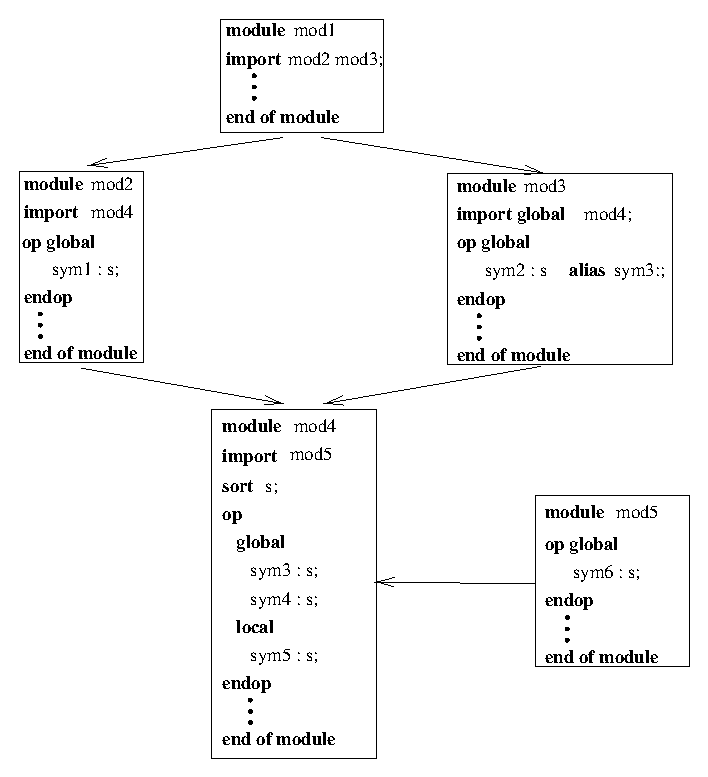
\psfig{figure=im_elan1.eps}
%%\end{minipage} \end{center}
%%In this situation:
%%\begin{itemize}
%%\item The sort {\tt s} is visible in all modules,
%%\item {\tt sym5} is visible only in {\tt mod4},
%%\item {\tt sym4} is visible in modules {\tt mod1}, {\tt mod2}, {\tt mod3}, and {\tt mod4},
%%\item {\tt sym3} is visible in the modules {\tt mod2}, {\tt mod3} and {\tt mod4} and it is
%%       also visible in {\tt mod1} but under the name {\tt sym2},
%%\item {\tt sym2} is just another name for {\tt sym3} and it is only visible in
%%        module {\tt mod1} and {\tt mod3},
%%\item {\tt sym1} is only visible in modules {\tt mod1} and {\tt mod2}.
%%\end{itemize}
%%\FEX
%%04-12-98 : l'exemple est dans l'ancienne syntaxe.

\subsection{Built-in modules}

For convenience and efficiency several modules are provided as
built-ins. See section~\ref{les built-in} for a full description of
the current available ones.

% the following modules are built-in
% \elan:
% \begin{enumerate}
%   \item {\tt anyInteger} provides the sort {\tt int} and all 
%           constants 0, 1, -1, 2, \ldots. A description of this module
%           is given in the standard library, see
%           page~\pageref{anyInteger module}.
%   \item {\tt anyIdentifier} provides the sort {\tt ident} and all 
%           constants a, b, c, aa, ab, \ldots. A description of this module
%           is given in the standard library, see
%           page~\pageref{anyIdentifier module}.
%   \item {\tt anyQuotedIdentifier} provides all quoted
%           constants ``a'', ``b'', ``c'', ``aa'', ``ab'', \ldots. A description
%           of this module is given in the standard library, see
%           page~\pageref{anyQuotedIdentifier module}.
% \end{enumerate}
% These modules can be imported as standard ones.

\subsection{Parameterised modules}

Parameterised modules can be defined in \elan\ as follows:

\grrule{formal module name}{
  \nt{identifier}
\gror
  \nt{identifier} \sym{[} \nt{identifier} \itzero{\sym{,}\nt{identifier}}
                  \sym{]}
}

The module instantiation by its actual parameters is currently done by
the syntactical replacement of the formal arguments by the actual ones.

\EX The classical example is the one of parameterised lists:\\
\insertExamples{simpleList.eln}

\noindent
and we get list of integers by 
instantiating {\tt X} by {\tt int} and importing {\tt int} as in:\\
\insertExamples{simpleList.lgi}
\FEX

%\EX [ck: Oct 29 97] exemple deja donne avant!
%Another classical example is based on the parameterised programming
%paradigm as advocated in~\cite{Goguen-HOF-unnecessary-90}:\\
%\insertExamples{map.eln}
%
%\FEX


\subsection{LGI modules}
\label{subsec.lgi.module}

The top level description of the logic consists of:
\begin{enumerate}
\item the description of the syntax that the user is allowed to use in
        order to give his specifications.
\item the description of a term, called the query, that will be reduced
        in the rewrite logic defined by the (super) user.
\end{enumerate}

The syntax is the following:
\grrule{lpl description}{
\rw{LPL} \nt{identifier} \rw{description}    \nl
\omm{\nt{specification description}}                  \nlp{5}
\rw{query}                                      \nlp{15}
        \rw{of sort} \nt{sort name}               \nlp{15}
        \rw{result of sort} \nt{sort name}       \nlp{15}
        \rw{import} \itone{\nt{instantiated module name}} \nlp{15}
        \omm{\rw{check with} \nt{boolean term}}         \nlp{15}
        \rw{start with} \nt{start term}          \nl
\rw{end}
}

\grrule{specification description}{
\rw{specification description}                  \nl
  \itone{\nt{specification part description}}   \nl
\rw{end}                                        
}

\grrule{specification part description}{
\rw{part} \nt{identifier}                 \nlp{10}
\rw{of sort} \nt{sort name}        \nlp{10}
\rw{import} \itone{\nt{instantiated module name}}        \nlp{10}
\omm{\rw{check with} \nt{boolean term}}   
}

\grrule{start term}{\sym{(} \omm{\nt{Estrategy name}} \sym{)} \nt{query term}}

The syntax of of \nt{query term} is built over the user-defined
signature enriched by the constant {\bf query}. The sort of {\bf
query} is given by the query declaration above.

\EX If no specification is needed, the specification description part
is skipped, as in the 
following logic description used for running
Example~\ref{testStrat.eln}:\\

\insertExamples{testStrat.lgi}
\FEX

\EX \label{unif.lgi.example}
Here is a simple example of the top level description of how unification can 
be implemented:\\
\insertExamples{unification.lgi}
\noindent
In this unification logic, the user should provide the specification
information as follows:\\
\insertExamples{simplesig.spc}

The user should use the (super-user defined) keywords {\tt Vars} and
{\tt Ops} to define respectively the variables and the operators,
namely {\tt a} of arity 0, {\tt f} of arity 2, etc...

\FEX

\subsubsection{Semantics}

When parsing a specification, \elan\ generates new modules that
 complete the definition of the rewrite theory to be used during the
 evaluation of the query. For instance, in the case of the previous
 example, these new modules are:
\\
\insertExamples{moduleVarUnif.eln}

\noindent
and\\
\insertExamples{moduleOpsUnif.eln}

When a user provides a specification to an \elan\ logic, this simply
provides more information about the context in which the user wants
to work, like the name of function symbols or basic axioms to use.

\section{Pre-processing}
\label{preprocessor}

Another original feature proposed by \elan\ is the use of a
pre-processing phase that allows to describe the logic to be encoded
in an easier way.

As described in Figure~\ref{elan-principle}, the pre-processor is
performing textual replacements starting from informations given by
the super-user in the modules, and by the user in the specification
file. The pre-processing phase in \elan\ can just be thought of as a
macro expansion mechanism which extends the parameterization process
described before.

In order to express the syntax of the pre-processor construction, we
need the notion of {\it constant expression} and of {\it text} defined
as follows:

\grrule{constant expression} {
        \nt{number}
\gror
        \sym{(}\nt{subexpression}\sym{)}
}

\grrule{subexpression} {
        \nt{number}
\gror
        \nt{subexpression} \sym{+} \nt{subexpression}
\gror
        \nt{subexpression} \sym{-} \nt{subexpression}
\gror
        \nt{subexpression} \sym{*} \nt{subexpression}
\gror
        \nt{subexpression} \sym{/} \nt{subexpression}
\gror
        \nt{subexpression} \sym{\%} \nt{subexpression}
\gror
        \sym{(}\nt{subexpression}\sym{)}
}

\grrule{lexem}{
      \nt{identifier}
\gror \nt{number}
\gror \nt{char}
}

\grrule{text}{\itone{\nt{lexem}}}

\subsection{Simple duplication}

A first feature is to allow simple duplications of a part of text. The
syntax is:

\grrule{simple repetition} {
  \nt{lexem}\symmm{$\tilde{\ }$}\nt{constant expression}
\gror
  \sym{\{} \nt{text} \sym{\}}\symmm{$\tilde{\ }$}\nt{constant expression}
}

\EX
The text ``$\tt a\{, b\}\tilde{\ }3$'' is processed into ``{\tt a, b,
b, b}''. 
\FEX

\subsection{Duplication with argument}

It is often necessary to allow description of objects like
$f(t_1,\ldots,t_5)$. This is possible using the syntax:


\grrule{arg.repetition}{
  \sym{\{} \nt{text} \sym{\}}\symmm{\_}
  \nt{identifier} \nl
  \sym= \nl
  \nt{constant expression} \sym{...} \nt{constant expression}}

\EX
The text ``{\tt P \{ \& s\_I=t\_I \}\_I=1...3}'' is processed into
``{\tt P  \& s\_1=t\_1 \& s\_2=t\_2  \& s\_3=t\_3}''. 
\FEX

A special form of this duplication with arguments is the explicit
construction of a list of indexed identifiers allowed using the
syntax:

\grrule{arg.repetition}{
  \nt{identifier}\symmm\_\nt{number}\nt{char}\sym{...}\nt{char}
  \nt{identifier}\symmm\_\nt{number}
}

\EX
The text ``{\tt t\_1,...,t\_5}'' is processed into ``{\tt t\_1 , t\_2
, t\_3 , t\_4 , t\_5}''. 
\FEX

\subsection{Enumeration using FOR EACH}\label{for each}

This construction allows to make the link between the specification
given by the user and the logic described by the super-user. A natural
motivation for this construction is given by the ``standard'' way
inference rules are used. For example when describing how unification
works, the following transformation rule is given:
\renewcommand{\fleche}{\ra}
\uneregle{Decompose}
        {P \ww \f{s}{n} \eqq \f{t}{n} }
        {P \ww s_1 \eqq t_1\ww \ldots \ww s_n \eqq t_n }
It is generic in the sense that the operator $f$ is unspecified. It
can be a $+$ of arity 2, or a $if@then@else@$ of arity 3, or just a
constant. We do not want, when specifying how the logic works, to give
only the specific cases, we need to be as generic as possible.

\elan\ provides via the FOR EACH construction of the pre-processor, a
way to be generic. The syntax is the following:

\grrule{for each const.} {
  \rw{FOR EACH} \nt{vardecl} \rw{SUCH THAT} \nt{varaffect} \sym{: \{}\nlp{5}
     \nt{text} \nl
  \sym{\}}
}

\grrule{vardecl}{
  \nt{varname}\itzero{\sym,\nt{varname}} \sym: \nt{sort name}
\gror
  \nt{vardecl}\sym;\nt{vardecl}
}

\grrule{varaffect}{
  \nt{varname} \sym{:= (} \omm{\nt{strategy name}} \sym) \nt{term}
\gror
  \nt{varaffect} \rw{AND} \nt{varaffect}
\gror
  \nt{varaffect} \rw{ANDIF} \nt{boolean term}
}

\Attention{
Since the symbols {\tt \{, \},$ \tilde{\ }$} are reserved for
pre-processor use, it is not possible to use them for any other
purpose, even quoted.
}

\Attention{
The pre-processor uses the character `\_' (underline) for assembling
identifiers. For example, the text `{\tt a f \_1\_ x b}'' is pre-processed
into the sequence of three identifiers {\tt a}, {\tt f\_1\_x} and {\tt
b}. The character `\_' is thus part of an identifier even if there is
a space between it and the rest of the string. It is thus better for
the user not to use the \_ symbol, except for building identifiers of course.
}

\EX
The rule \rname{Decompose} that we mentioned at the beginning of
this section can be expressed in the following way:\\
\insertExamples{decomposition.eln}

If the specification given by the user consists in the operator symbols
{\tt f} and {\tt g} of respective arities 2 and 1, then the
pre-processor expands the previous {\bf FOR EACH} construction into:\\
\insertExamples{decompositionExpanded.eln}

\FEX


\section{Differences with previous version of the language}
\label{versionChanges}

The language has evolved a lot between \elan\ version 1.17 and \elan\
version 3.0. The changes concern the syntax of:
\begin{itemize}
  \item modules,
  \item rules and
  \item strategies.
\end{itemize}

The main changes are emphasized in the corresponding sections of the
language description, and the main concern has been to uniformize the
language constructions.

The transformations needed to change from the syntax of version 1.17 to the
current one (i.e. later than 2.00) are summarized below.

Concerning the declaration parts:
\begin{itemize}
\item \texttt{import ...} becomes \texttt{import ... end}
\item \texttt{sort ...} becomes \texttt{sort ... end}
\item \texttt{op ... endop} becomes \texttt{operators ... end}
\end{itemize}
Now, there is only one construction to define rules, you have to
replace: 
\begin{itemize}
\item \texttt{rule for ...} by \texttt{rules for ...}
\item \texttt{rule <name> for ...} by \texttt{rules for ... [name] ...}
\item suppress \texttt{declare} keyword
\item \texttt{body} or \texttt{bodies} by \texttt{global} or
  \texttt{local}
\item \texttt{end of rule}, \texttt{end of rules} by \texttt{end}
\end{itemize}

The rule labels accept now arguments that should be variables involved
in the rule.

Definition of strategies looks like rules definitions, you have to
replace: 
\begin{itemize}
\item \texttt{strategy ...} by \texttt{strategies for ... global|local
    [name] ...} 
\item \texttt{iterate ... enditerate} by \texttt{iterate*(...)}
\item \texttt{while ... endwhile} by \texttt{repeat*(...)}
\item \texttt{repeat ... endrepeat} by \texttt{repeat*(...)}
\item \texttt{dont know choose(...)} by \texttt{dk(...)}
\item \texttt{dont care choose(...)} by \texttt{dc(...)}
\item \texttt{end of strategy} by \texttt{end}
\item \texttt{end of module} by \texttt{end}
\end{itemize}
Local affectations and conditions are now evaluated from top to
bottom. The order of presentation has been reversed, so that the {\em
old} syntax:
\begin{verbatim}
  [] l => r
          if c2
          where v2:=(...) ...
          where v1:=(...) ...
          if c1
\end{verbatim}
becomes in the {\em new} syntax:
\begin{verbatim}
  [] l => r
          if c1
          where v1:=(...) ...
          where v2:=(...) ...
          if c2
\end{verbatim}

